\chapter{Electrostatics, Part 1 (Point Charges)}
\label{chapter:electrostatics1}


\section{Electric Charge}

From the onset, we know that there are two types of charge, which we have
assigned a positive or negative sign to facility mathematical calculations.

The SI unit of charge is a \emph{coulomb}, which is defined as the amount of
charge that one \emph{amp\`{e}re} of current passing through a circuit in one
second:
\begin{equation*}
  \SI1\coulomb=\SI1\ampere\cdot\SI1\second
\end{equation*}
At this time, we have not defined what an amp\`{e}re of current is. It is one
of the seven base SI units, and it is defined based on the magnetic force that
two current-carrying wire exert on each other.

With the development of atomic theory in the beginning of the 20th Century, we
understand that there are two stable elementary particles that carry an
electrical charge. The positive charge is carried by the proton, while the
negative the charge is carried by the electron. The proton is inside the
nucleus of the atom, while the electron orbits around the nucleus.

%    \begin{center}
%      \textbf{Proton}
%    \end{center}
%    \begin{itemize}
%    \item Mass: $m_p=\SI{1.673e-27}{\kilo\gram}$
%    \item Charge: $e^+=+\SI{1.602e-19}\coulomb$
%    \end{itemize}
%
%    \begin{center}
%      \textbf{Electron}
%    \end{center}
%    \begin{itemize}
%    \item Mass: $m_e=\SI{9.109e-31}{\kilo\gram}$
%    \item Charge: $e^-=\SI{-1.602e-19}\coulomb$
%    \end{itemize}


Although the mass of the electron and the proton are different, they both carry
the same amount of charge, called the elementary charge $e$, with a value of
\begin{equation*}
  e=\SI{-1.602e-19}\coulomb
\end{equation*}
The proton carries a charge of $+e$, while the electron carries a charge of
$-e$.

A ``charge particle'' $q$ may be a single electron, a single proton, an ion, or
any object that has an imbalance of protons and electrons. The total charge of
an object is the difference between the number of protons ($N_\text{proton}$) and
electrons ($N_\text{electron}$), multiplied by the elementary charge $e$:
\begin{equation}
  q=e|N_\text{proton}-N_\text{electrons}|
\end{equation}



\section{Coulomb's Law for Electrostatic Force}

We will begin with \textbf{electrostatics}, where charges that are not moving
(or moving slowly) relative to one another

Electric charges exert an \textbf{electrostatic force}\footnote{Also known as
the \textbf{electric force}, or the \textbf{coulomb force}. It is a
fundamental force; and also a conservative force.} $\bm F_q$ on each other.
The direction of the force is based on the \emph{sign} of the charges:
\begin{itemize}
\item Like charges \emph{repel} (positive \& positive; negative \& negative)
\item Opposite charges \emph{attract} (positive \& negative)
\end{itemize}
as shown in Fig.~\ref{fig:coulomb-charge}.
\begin{figure}[ht]
  \centering
  \begin{subfigure}{.7\linewidth}
    \centering
    \begin{tikzpicture}[scale=.6]
      \draw[vectors] (0,0)--(2,0) node[above]{$\bm F_q$};
      \draw[vectors] (6,0)--(4,0) node[above]{$\bm F_q$};
      \draw[poscharge] circle (.4) node[white]{$\bm +$};
      \draw[negcharge] (6,0) circle (.4) node[white]{$\bm -$};
    \end{tikzpicture}
    \caption{Electrostatic force between opposite charges is attractive}
  \end{subfigure}
  
  \begin{subfigure}{.7\linewidth}
    \centering
    \begin{tikzpicture}[scale=.6]
      \draw[vectors] (0,0)--(-2.5,0) node[above]{$\bm F_q$};
      \draw[vectors] (2.5,0)--(5,0) node[above]{$\bm F_q$};
      \draw[poscharge] circle (.4) node[white]{$\bm +$};
      \draw[poscharge] (2.5,0) circle (.4) node[white]{$\bm +$};
    \end{tikzpicture}
    \caption{Electrostatic force between two positive charges is repulsive}
  \end{subfigure}
  
  \begin{subfigure}{.7\linewidth}
    \centering
    \begin{tikzpicture}[scale=.6]
      \draw[vectors] (0,0)--(-2.5,0) node[above]{$\bm F_q$};
      \draw[vectors] (2.5,0)--(5,0) node[above]{$\bm F_q$};
      \draw[negcharge] circle (.4) node[white]{$\bm -$};
      \draw[negcharge] (2.5,0) circle (.4) node[white]{$\bm -$};
    \end{tikzpicture}
     \caption{Electrostatic force between two negative charges is repulsive}
  \end{subfigure}
  \caption{Electrostatic force between charged particles}
  \label{fig:coulomb-charge}
\end{figure}

The magnitude of the electrostatic force between two \emph{point charges} is
given by \textbf{Coulomb's law}:
\begin{important-equation}
  F_q=\frac{k\left|q_1q_2\right|}{r^2}
  \label{eq:coulombs-law}
\end{important-equation}

where $k$ is called \textbf{Coulomb's constant},with a value of
\begin{equation*}
  k=\SI{8.99e9}{\newton\metre\squared\per\coulomb\squared}
\end{equation*}
Coulomb's law is defined based on another fundamental constant called the
\textbf{permittivity of free space}, or \textbf{vacuum permittivity}
($\varepsilon_0$):
\begin{important-equation}
  k=\frac1{4\pi\varepsilon_o}
\end{important-equation}
Permittivity of free space is a measure of how well a vacuum can resist the
formation of an electric field, with a value of
\begin{equation*}
  \varepsilon_0=\SI{8.85e-12}{C^2/N.m^2}
\end{equation*}
A vacuum is not particularly good at resisting electric fields from forming,
hence the very small value of $\varepsilon_0$. However, inside dielectric
materials, the effective permittivity would be much higher.

Like the point mass model used in the law of universal gravitation, in
Coulomb's law, charges $q_1$ and $q_2$ are also assumed to be
\emph{point charges} that do not occupy any space. In reality, of course, point
charges do not actually exist, therefore $r$ cannot be zero, and $\bm F_q$
cannot be infinitely large. But whether you can treat a charge as a point
charge is a matter of scale. If the charge is the size of an electron or a
proton, then even at the scale of the atom. However, if the charge is a large
piece of metal of irregular shape, then the point-charge model would be very
inaccurate near the charge. Additionally, using the point charge model for
charges, we must also assume that one charge is not inside another.

As is the case for \emph{all} forces, the electrostatic force obeys the third law
of motion: if $q_1$ exerts an electrostatic force $\bm F_q$ on $q_2$, then
$q_2$ likewise exerts a reaction force of $-\bm F_q$ on $q_1$. The two
forces are equal in magnitude and opposite in direction.

Coulomb's law has a very similar form to the law of universal
%gravitation (Eq.~\ref{eq:law-of-gravity}).
gravitation.
The major difference is that whereas masses are \emph{always} positive, and the
gravitational force is \emph{always} attractive, charges can be either positive
or negative, and therefore the electrostatic force may be attractive or
repulsive. Nevertheless, much of the analysis used


%\section{Review: The Charges Are}
%We should already know a bit about charge particles:
%\begin{itemize}
%\item A \textbf{proton} carries a \textbf{positive} charge
%\item An \textbf{electron} carries a \textbf{negative} charge
%\item A \emph{net charge} of an object means an excess of protons or electrons
%\item Similar charges are repel; opposite charges attract
%\end{itemize}
%
%\vspace{.2in}We start with electrostatics:
%\begin{itemize}
%\item Charges that are not moving relative to one another
%\end{itemize}
%
%The SI unit for electric charge is a \emph{coulomb}, which is the amount of
%charges that flows through a circuit



%\section{Coulomb's Law for Electrostatic Force}
%\begin{center}
%  \begin{tikzpicture}[scale=.65]
%    \draw[vector,red] (0,0)--(2,0) node[right]{$\bm F_q$};
%    \draw[vector,blue] (8,0)--(6,0) node[left] {$\bm F_q$};
%    \shade[ball color=red] circle (.2) node[above]{$q_1$};
%    \shade[ball color=blue] (8,0) circle (.2) node[above]{$q_2$};
%    \draw[dashed] (0,0)--(0,-1.5);
%    \draw[dashed] (8,0)--(8,-1.5);
%    \draw[vector] (0,-1.3)--(8,-1.3) node[midway,below]{$\bm r_{12}$};
%  \end{tikzpicture}
%\end{center}
%The \textbf{electrostatic force}\footnote{It is also known as the
%\textbf{electric force} or \textbf{coulomb force} in different textbooks and
%technical journals. We will use these terms interchangeably throughout the
%course.} $\bm F_q$ is a mutually repulsive/attractive force between all
%charged objects. The force that point charge $q_1$ exerts on $q_2$ is given
%by \textbf{Coulomb's law}:
%
%\begin{equation}
%  \boxed{\bm F_q=\frac{kq_1q_2}{|\bm r_{12}|^2}\hat{\bm r_{12}}}
%\end{equation}
%
%
%
%
%
%\section{Coulomb's Law for Electrostatic Force}
%\begin{equation}
%  \boxed{
%    \bm F_{12}=\frac{kq_1q_2}{|\bm r_{12}|^2}\hat{\bm r_{12}}
%  }
%\end{equation}
%\begin{center}
%  \begin{tabular}{l|c|c}
%    \rowcolor{pink}
%    \textbf{Quantity} & \textbf{Symbol} & \textbf{SI Unit} \\ \hline
%    Electrostatic force    & $\bm F_{12}$ & \si\newton \\
%    Coulomb's constant & $k$ &
%    \si{\newton\metre\squared\per\coulomb\squared}\\
%    Point charges 1 and 2  & $q_1$, $q_2$ &  \si\coulomb \\
%    Distance between point charges & $|\bm r_{12}|$ & \si\metre \\
%    Unit vector of direction between point charges & $\hat{\bm r_{12}}$ &
%  \end{tabular}
%\end{center}
%
%
%
%
%\section{Coulomb's Constant}
%\begin{equation}
%  \boxed{\bm F_{12}=\frac{kq_1q_2}{|\bm r_{12}|^2}\hat{\bm r_{12}}}
%\end{equation}
%
%The constant $k$ in the Coulomb's law is called the
%\textbf{coulomb's constant}, defined as:
%\begin{equation}
%  k=\dfrac1{4\pi\epsilon_0}=
%  \SI{8.99e9}{\newton\metre\squared\per\coulomb\squared}
%\end{equation}
%where $\epsilon_0$ is a fundamental constant called the
%\textbf{permittivity of free space}, or \textbf{vacuum permittivity}. It
%measures a vacuum's ability to resist the formation of an electric field:
%\begin{equation}
%  \epsilon_0=\SI{8.85e-12}{C^2/N.m^2}
%\end{equation}
%
%
%
%\section{Coulomb's Law for Electrostatic Force}
%\begin{center}
%  \begin{tikzpicture}[scale=.5]
%    \draw[vector,red] (0,0)--(2,0) node[right]{$\bm F_{12}$};
%    \draw[vector,blue] (8,0)--(6,0) node[left] {$\bm F_{21}$};
%    \shade[ball color=red] circle (.2) node[above]{$q_1$};
%    \shade[ball color=blue] (8,0) circle (.2) node[above]{$q_2$};
%    \draw[dashed] (0,0)--(0,-1.5);
%    \draw[dashed] (8,0)--(8,-1.5);
%    \draw[axes] (0,-1.3)--(8,-1.3) node[midway,below]{$\bm r_{12}$};
%  \end{tikzpicture}
%\end{center}
%\begin{itemize}
%\item Third law of motion: If $q_1$ exerts an electrostatic force
%  $\bm F_{12}$ on $q_2$, then $q_2$ likewise exerts a force of
%  $\bm F_{21}=-\bm F_{12}$ on $q_1$. The two forces are equal in magnitude
%  and opposite in direction.
%\item $q_1$ and $q_2$ are assumed to be \emph{point charges} that do not
%  occupy any space
%\item The scalar form is often used as well, since the direction of $F_q$ can
%  easily be found:
%  \begin{equation}
%    \boxed{F_q=\frac{kq_1q_2}{r^2}}
%  \end{equation}
%\end{itemize}


%\section{More Than One Charge}
\begin{figure}[H]
  \centering
  \begin{tikzpicture}[scale=.37]
    \shade[ball color=red] circle (.72) node[white]{$Q$};
    
    \begin{scope}[rotate=45]
      \draw[vector,blue] (.72,0)--(2.5,0) node[right]{$\bm F_1$};
      \shade[ball color=blue] (7,0) circle (1) node[white]{$q_1$};
    \end{scope}
    
    \begin{scope}[rotate=105]
      \draw[vector,green] (.72,0)--(2,0) node[right]{$\bm F_2$};
      \shade[ball color=green] (4,0) circle (.65) node[white]{$q_2$};
    \end{scope}
    
    \begin{scope}[rotate=190]
      \draw[vector,yellow] (.7,0)--(3.5,0) node[above]{$\bm F_3$};
      \shade[ball color=yellow!70!black] (6,0) circle (1.1) node[white]{$q_3$};
    \end{scope}
    
    \begin{scope}[rotate=260]
      \draw[vector,violet] (.72,0)--(1.4,0) node[right]{$\bm F_4$};
      \shade[ball color=violet] (9,0) circle (.8) node[white]{$q_4$};
    \end{scope}
    
    \begin{scope}[rotate=125]
      \draw[->,ultra thick](.72,0)--(3.5,0) node[left]{$\bm F$};
    \end{scope}
  \end{tikzpicture}
  \caption{A charge $Q$ subjected to multiple electric forces}
  \label{fig:multiple-charges-force}
 \end{figure}
For a charge $Q$ that is subjected to the influence of multiple discrete
point charges $q_i$, such as the example in
Fig.~\ref{fig:multiple-charges-force}, the total electrostatic force that $Q$
experiences is the vector sum of all the forces $\bm F_i$:
\begin{important-equation}
  \bm F
  =\sum_i\bm F_i
  =kQ\left(\sum_{i=1}^N\frac{q_i}{r_i^2}\hat{\bm r_i}\right)
\end{important-equation}
As $N\rightarrow\infty$, the summation becomes an integral, and can now be
used to describe the force from charges with \emph{spatial extend} i.e.\
charges that take up physical space (e.g.\ a continuous distribution of
charges):
\begin{important-equation}
  \bm F
  =\int\dl{\bm F}
  =kQ\int\frac{\dl q}{r^2}\hat{\bm r}
\end{important-equation}



There is a net force that acts on $Q$, therefore it will accelerate (second
law of motion) with an acceleration of
\begin{equation*}
  a=\frac{\bm F_\text{tot}}{m_Q}
\end{equation*}
where $m_Q$ is the mass of charge $Q$. However, we note that even if
$q_1,\ldots,q_N$ remain stationary, as soon as $Q$ moves, all the forces acting
on it (and therefore its acceleration) will change in both magnitude and
direction. In general, predicting the motion of $Q$ is difficult because of the
changing forces and acceleration, even with calculus.


\subsection{Infinitesimal Charge}
\label{section:charge-density}

Expressions for infinitesimal charge $\dl q$ is similar to the infinitesimal
mass $\dl m$ concept discussed earlier in Chapter~\ref{chapter:cm}:
\begin{itemize}
\item Linear charge density (for 1D problems)
  \begin{equation}
    \gamma(x) = \diff qx\quad\rightarrow\quad \dl q =\gamma(x)\dl x
  \end{equation}
  \item Surface charge density (for 2D problems)
    \begin{equation}
      \sigma(x,y)=\diff qA\quad\rightarrow\quad \dl q=\sigma(x,y)\dl A
    \end{equation}
  \item Charge density (for 3D problems)
    \begin{equation}
      \rho(x,y,z)=\diff qV\quad\rightarrow\quad \dl q=\rho(x,y,z)\dl V
    \end{equation}
\end{itemize}

\begin{remark}
  Let's be careful here. The Greek letter \emph{rho} ($\rho$) is used in
  different contexts in this book. Throughout Part~\ref{part:mechanics} of
  this book, it is used exclusively for mass density.
  %in Chapter~\ref{chapter:cm}.
  Here, we are using it for \emph{charge} density (charge per unit volume).
  Later, in Chapter~\ref{chapter:circuits}, we will use the same symbol for
  resistivity of a material. It is important that we don't get mixed up with
  the notation.
\end{remark}

    
\section{Electric Field}
In light of our new knowledge of the coulomb's law in
Eq.~\ref{eq:coulombs-law}, and its similarity to the law of universal
gravitation in Eq.~\ref{eq:universal-grav}, the expression for
\textbf{electric field} $\bm E$ can be obtained by repeating the same procedure
as with gravitational field, by grouping the variables in Coulomb's law:
\begin{equation}
  F_q
  =\underbrace{
    \left[\frac{kq_1}{|\bm r_{12}|^2}\hat{\bm r}\right]
  }_{\bm E}q_2
\end{equation}
Just as the gravitational field is a vector function that shows how a mass
influences the gravitational forces on other masses in its vicinity, here, the
electric field function $\bm E$ created by $q_1$ shows how it influences the
electrostatic forces on other charged particles in its vicinity.

The electric field a distance $r$ away from a point charge $q$ is given by:
\begin{important-equation}
  \bm E(q,\bm r)=\frac{kq}{r^2}\hat{\bm r}
   \quad\text{(point charge)}
  \label{eq:pt-charge-E}
\end{important-equation}
%\begin{center}
%  \begin{tabular}{l|c|c}
%    \rowcolor{pink}
%    \textbf{Quantity} & \textbf{Symbol} & \textbf{SI Unit} \\ \hline
%    Electric field intensity    & $\bm E$ & \si{\newton\per\coulomb}\\
%    Coulomb's constant          & $k$   & \si{N.m^2/C^2} \\
%    Source charge               & $q$   & \si\coulomb \\
%    Distance from source charge & $r$ & \si\metre \\
%    Radially outward direction from point source & $\hat{\bm r}$ &
%  \end{tabular}
%\end{center}
The direction of $\bm E$ is radially outward from a positive point charge
and radially inward toward a negative charge. The SI unit for electric field
is \textbf{newton per coulomb} (\si{\newton\per\coulomb}) or
\textbf{volt per meter} (\si{\volt\per\metre}). Both units are equivalent,
and both are used in AP exams.

When multiple discrete point charges are present, the total electric field at
any position $\bm r$ is the vector sum of all the fields $\bm E_i$:
\begin{important-equation}
  \bm E
  =\sum_i\bm E_i
  =k\left(\sum_{i=1}^N\frac{q_i}{r_i^2}\hat{\bm r_i}\right)
   \quad\text{(multiple point charges)}
\end{important-equation}
As $N\rightarrow\infty$, the summation becomes an integral, and can now be
used to describe the electric field generated by \emph{charge distributions
with spatial extend}:
\begin{important-equation}
  \bm E=\int\dl{\bm E}=k\int\frac{\dl q}{r^2}\hat{\bm r}
  \quad\text{(continuous charge distribution)}
\end{important-equation}
Like the integration for the electrostatic force, integrating $\bm E$ is also
difficult if the geometry is complex or irregular.
%In general, this integral is difficult to evaluate for complex geometries.
%but in AP Physics C, we can usually exploit symmetry.


$\bm E$ itself \emph{doesn't do anything} until another charge interacts with
it. And when there is a charge $q$, the electrostatic force $\bm F_q$ that
the charge experiences is proportional to $q$ and $\bm E$, regardless of how
the electric field is generated\footnote{Analogous to the relationship
for gravity: $\bm F_g=m\bm g$}:
\begin{important-equation}
  \bm F_q=q\bm E
\end{important-equation}
A positive charge in the electric field experiences an electrostatic force
$\bm F_q$ in the same direction as $\bm E$; a negative charge experiences
a force in the opposite direction as $\bm E$.




\section{Electric Field Lines}
\textbf{Electric field lines} can be used to visualize the direction of the
electric field. For point charges:
\begin{center}
  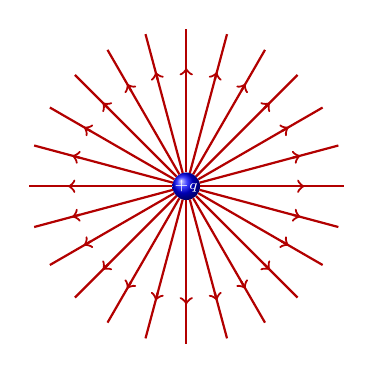
\begin{tikzpicture}[scale=.5]
    \shade[ball color=blue] circle (.35) node[white]{\tiny $+q$};
    \foreach \theta in {15,30,...,360}{
      \begin{scope}[rotate=\theta,red!70!black,thick]
        \draw[->] (.35,0)--(3,0);
        \draw (2.8,0)--(4,0);
      \end{scope}
    }
  \end{tikzpicture}
  \hspace{.2in}
  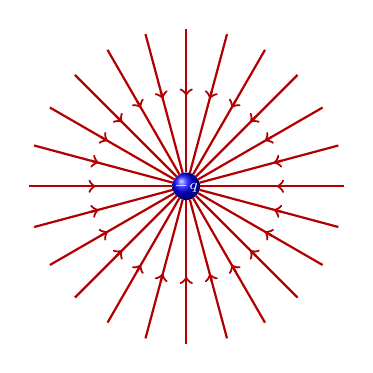
\begin{tikzpicture}[scale=.5]
    \shade[ball color=blue] circle (.35) node[white]{\tiny $-q$};
    \foreach \theta in {15,30,...,360}{
      \begin{scope}[rotate=\theta,red!70!black,thick]
        \draw (.35,0)--(2.5,0);
        \draw[<-] (2.3,0)--(4,0);
      \end{scope}
    }
  \end{tikzpicture}
\end{center}




\begin{center}
  \pic{.8}{electrostatics/field-lines}
\end{center}
\begin{itemize}
\item Electric field lines must begin and/or end at a charge
\item Field lines do not cross
\item Direction of the electric field is tangent to the field lines
\end{itemize}




\subsection{Electric Field Along Axis of a Ring Charge}

Suppose you have been given \emph{The One Ring To Rule Them All}, and you
found out that it is charged! What is its electric field at point $P$ along
its axis?
\begin{center}
  \pic{.5}{electrostatics/physicsbook_emism_graphik_35}
\end{center}
Note that calculating the electric field away from the axis is very
difficult.






\begin{center}
  \pic{.5}{electrostatics/Fig25}
\end{center}

\begin{itemize}
\item We can separate the electric field $\dl{\bm E}$ (generated by charge
  $\dl q$) into axial ($\dl E_x$) and radial ($\dl E_\perp$) components
\item Based on symmetry, $\dl E_\perp$ doesn't contribute to anything; but
  $\dl E_x$ is pretty easy to find:
\end{itemize}
\begin{equation}
  \dl E_x =\frac{k\dl q}{r^2}{\color{red}\cos\theta}
  =\frac{k\dl q}{r^2}{\color{red}\frac xr}
  =\frac{kx\dl q}{(x^2+a^2)^{3/2}}
\end{equation}
Integrating this over all charges $\dl q$, we have:
\begin{equation} 
    E_x          
    =\int \dl E_x       
    =\frac{kx}{(x^2+a^2)^{3/2}}\int \dl q=\boxed{\frac{kQx}{(x^2+a^2)^{3/2}}}
\end{equation}                     




\subsection{Electric Field Along Axis of a Uniformly Charged Disk}
Let's extend what we know to a disk of radius $a$ and charge density $\sigma$
\begin{center}
  \pic{.5}{electrostatics/serway}
\end{center}
  
We start with the solution from the ring problem, and replace $Q$ with
$\dl q=2\pi\sigma r\dl r$:
\begin{equation}
  \dl E_x =\frac{2\pi kr\sigma x}{(x^2+r^2)^{3/2}}\dl r
\end{equation}
Integrating over the entire disk:
\begin{equation}
  E_x =\pi kx\sigma\int_0^a\frac{2r}{(x^2+r^2)^{3/2}}\dl r
\end{equation}
This is not an easy integral!

Luckily for us, the integral is in the form of $\int u^n\dl u$,
with $u=x^2+r^2$ and $n=\frac{-3}2$. You can find the integral in any math
textbook:

\begin{equation}
  E_x =2\pi k\sigma\left(1-\frac x{\sqrt{x^2+a^2}}\right)
\end{equation}
  

\section{Electric Potential Energy}
If an electrostatic force acts on a charge, and if the charge moves, then we
can calculate the work done by the electrostatic force. Bear in mind that as
this charge moves, then both the magnitude and direction of $\bm F_q$ are
likely to change. Therefore, calculating the work done generally requires
integrating the electrostatic force along the path $\mathcal S$ of the charge,
from position $r_0$ to $r_1$:
%The electrostatic force is a conservative force; 
\begin{equation}
  W_q=\int_{\mathcal S}\bm F_q\cdot\dl{\bm r}
  =kq_1q_2\int_{r_0}^{r_1}\frac{\dl r}{r^2}
  =-\frac{kq_1q_2} r\Big|^{r_1}_{r_0}=-\Delta U_q
\end{equation}
The work done by $\bm F_q$ is related to the change in
\textbf{electric potential energy} $U_q$, which is the energy stored between a
system of two charges. It is defined as:
\begin{important-equation}
  U_q=\frac{kq_1q_2}r
  \label{eq:Uq}
\end{important-equation}
Similar gravitational potential energy (Eq.~\ref{eq:real-Ug}),
Eq.~\ref{eq:Uq} uses  $r=\infty$ as the reference\footnote{The \emph{reference}
is where $U=0$ by definition}. However, unlike gravitational potential energy
which is \emph{always} negative, $U_q$ can be either positive or negative,
because charges can be either positive or negative. When $U_g>0$ (energy stored
between two positive charges or two negative charges), external work must be
done to bring the charges from $r=\infty$ to $r$. Conversely, if $U_q<0$
(energy stored between one positive and one negative charge), external work is
done to pull two charges apart from $r$ to $r=\infty$.
\begin{definition}
  \begin{enumerate}[leftmargin=15pt]
  \item When the work done by $\bm F_q$ is \emph{positive}, there is a
    \emph{decreases} in electric potential energy by the same amount
  \item When the work done by $\bm F_q$ is \emph{negative}, there is an
    \emph{increases} in electric potential energy by the same amount
  \item Work done is path independent: $W_q$ depends on the end points $r_1$ and
    $r_2$, but not \emph{how} the charges move from $r_1$ to $r_2$
  \item Only work done by $\bm F_q$ can change $U_q$
  \end{enumerate}
\end{definition}


%%\subsection{How it Differs from Gravitational Potential Energy}
%$U_q$ can be ($+$) or ($-$), because charges can be either ($+$) or ($-$)
%
%Two positive charges:
%
%\begin{equation}
%  U_q>0
%\end{equation}
%    
%Two negative charges:
%
%\begin{equation}
%  U_q>0
%\end{equation}
%    
%One positive and one negative charge:
%
%\begin{equation}
%  U_q<0
%\end{equation}
%  
%\begin{itemize}
%\item $U_q>0$ (both charges have the same sign): work is done to bring two
%  charges together from $r=\infty$ to $r$
%\item $U_q<0$ (the charges are opposite signs): work is done to separate the
%  two charges from $r$ to $r=\infty$
%\item Gravitational potential $U_g$ is always $<0$ because mass can only be
%  positive
%\end{itemize}




%\section{Relating $U_q$ to $\bm F_q$}
%From the fundamental theorem calculus, we can relate electrostatic force
%($\bm F_q$) to electric potential energy ($U_q$) by the gradient operator:
%
%\begin{equation}
%  U_q=-\int\bm F_q\cdot\dl{\bm r}\quad\rightarrow\quad
%  \bm F_q(r)=-\nabla U_q=-\diffp{U_q}r\hat{\bm r}
%\end{equation}
%Electrostatic force $\bm F_q$ always points from high to low potential
%energy (steepest descent direction)




\subsection{Potential Energy with More Than Two Charges}
When there are more than two charges, the total potential energy is the
total between the systems of 2 charges:

\begin{center}
  \begin{tikzpicture}[scale=1.3]
    \draw (0,0)--(1,-2) node[midway,right]{$r_3$}
    --(-3,-2) node[midway,below]{$r_2$} -- (0,0) node[midway,left=3]{$r_1$};
    \draw[mass] circle (.2) node{$q_1$};
    \draw[mass] (1,-2) circle (.2) node{$q_3$};
    \draw[mass] (-3,-2) circle (.2) node{$q_2$};
  \end{tikzpicture}
\end{center}

\begin{equation}
  U_q=\frac{kq_1q_2}{r_1} +\frac{kq_2q_3}{r_2} +\frac{kq_1q_3}{r_3}
\end{equation}
The energy stored can be either positive or negative depending on the sign of
the charges of $q_1$, $q_2$ and $q_3$.


\begin{example}
  Four identical charges $q$ are located at the four corners of a square of
  length $L$. What is the total potential energy of the system?
  \begin{center}
    \begin{tikzpicture}[scale=1.3]
      \draw rectangle (2,2) node[midway,above=35]{$L$};
      \draw[poscharge] (0,2) circle (.15) node[white]{$q$};
      \draw[poscharge] (0,0) circle (.15) node[white]{$q$};
      \draw[poscharge] (2,0) circle (.15) node[white]{$q$};
      \draw[poscharge] (2,2) circle (.15) node[white]{$q$};
    \end{tikzpicture}
  \end{center}
\end{example}



\section{Electric Potential}

An object at a specific location inside a gravitational field has a
gravitational potential energy proportional to its mass, i.e.\
\begin{equation}
    U_g=V_gm
\end{equation}
This ``constant'' $V_g$ is called the \textbf{gravitational potential}, which
is defined as \emph{gravitational potential energy per unit mass}. In the
simple case with a uniform gravitational field:
\begin{equation}
  V_g(h)=\frac{U_g}m=gh
\end{equation}
In the general case for the gravitational potential energy stored between
$M$ and $m$, we can define the gravitational potential from ``source mass''
$M$:
\begin{equation}
  V_g=\frac{U_g}m=-\frac{GM}r
\end{equation}
When $m$ is in this potential $V_g$, the gravitational potential energy is:
\begin{equation}
  U_g=V_gm=-\frac{GMm}r
\end{equation}
In agreement with the previous equations


This is also true for a charged particle $q$ in an electric field
created by $q_s$. In this case, the potential (the ``constant'') is called the
\textbf{electric potential}. The unit for electric potential is a \emph{volt}
which is \emph{one joule per coulomb}, i.e.\
$\SI1\volt=\SI1{\joule\per\coulomb}$
\begin{equation}
  \boxed{
    V=\frac{U_q}q
  }
\end{equation}
The electric potential from a source \underline{\emph{point}} charge $q_s$ is
therefore:
\begin{important-equation}
  V=\frac{kq_s}r
  \quad\text{from a point charge}
\end{important-equation}




%\section{Electric Potential: Point Charges}
  
\begin{center}
  \centering
  \begin{tikzpicture}[scale=.75]
    \shade[ball color=blue] circle (.3) node[white]{\tiny$\bm{+q}$};
    \foreach \theta in {20,40,...,360}{
      \draw[rotate=\theta,axes,gray] (.3,0)--(3,0);
      \draw[rotate=\theta,thick,gray] (2.8,0)--(4,0);
    }
    \foreach \r in {1,2,3}{
      \draw[very thick,red] circle (\r);
      \node[red,below] at (0,-\r+.09){$V_\r$};
    }
  \end{tikzpicture}
\end{center}

For a point charge $q$, every point at a distance $r$ has the same
electric potential $V$.
\begin{itemize}
\item The red lines have the same electric potential; they are called
  \textbf{equipotential lines}, or \textbf{equipotential contours}
\item Equipotential lines are perpendicular to the electric field lines
\item Electric field lines always points from higher $V$ toward lower $V$
\end{itemize}
\begin{equation}
  V_1>V_2>V_3
\end{equation}
  
  %\vspace{.1in}In AP Physics C, equipotential contours are sometimes also known
  %as \textbf{isolines of equal electric potential}.


  
\begin{center}
  \centering
  \begin{tikzpicture}[scale=.75]
    \shade[ball color=blue] circle (.3) node[white]{\tiny$\bm{+q}$};
    \foreach \theta in {20,40,...,360}{
      \draw[rotate=\theta,axes,gray] (.3,0)--(3,0);
      \draw[rotate=\theta,gray,thick] (2.8,0)--(4,0);
    }
    \foreach \r in {1,2,3}{
      \draw[very thick,red] circle (\r);
      \node[red,below] at (0,-\r+0.09){$V_\r$};
    }
    \shade[ball color=red,rotate=-20] (2,0) circle (.23) node[white]{$Q$};
  \end{tikzpicture}
\end{center}
A charge $Q$ that is placed inside this electric field has an electric
potential energy of:
\begin{equation}
  U_q=QV=Q\left[\frac{kq}r\right]
\end{equation}  
in agreement with equation for electric potential energy
  





%\section{Electric Potential from Multiple Charges}
When multiple discrete point charges are present, the total electric
potential is given by the summation\footnote{Note that this is scalar
summation!}:

\begin{important-equation}
  V =k\sum_{i=1}^N\frac{q_i}{r_i}
\end{important-equation}
As $N\rightarrow\infty$, the summation becomes an integral, and we can use it
to evaluate the potential from a continuous distribution of charges:
\begin{important-equation}
  V =k\int\frac{\dl q}r
\end{important-equation}
  %where $r$ is the distance to the infinitesimal charge $\dl q$




\fcolorbox{black}{yellow!10}{
  \small
  \begin{minipage}{.97\linewidth}
    \begin{center}
      \begin{tikzpicture}
        \draw[axes] (-2,0)--(2,0) node[right]{$x$};
        \draw[axes] (0,-2)--(0,2) node[right]{$y$};
        \draw[gray] circle (1.5);
        \draw[line width=2,red,rotate=90] (1.5,0) arc (0:180:1.5)
        node[pos=.25,above=3]{$Q$};
      \end{tikzpicture}
    \end{center}
    \textbf{Example:} A uniform charge $Q$ is located
    \begin{enumerate}[nosep]
      %\item What is the electric field at the origin?
    \item What is the electric potential at the origin?
    \item A charge $q$ is moved from $x=\infty$ to the origin. What is the
      work done?
    \end{enumerate}
  \end{minipage}
}
  




%\section{Relating $V$ to $\bm E$}
%In the same way that the fundamental theorem of calculus relates the 
%electrostatic force ($\bm F_q$) and electric potential energy ($U_q$) by the
%gradient operator, electric field ($\bm E$) and electric potential ($V$) are
%also related the same way:
%
%\begin{equation}
%  V(r)=-\int\bm E(r)\cdot\dl{\bm r}\quad\rightarrow\quad
%  \bm E(r)=-\nabla V(r)=-\diff Vr\hat{\bm r}
%\end{equation}
%\begin{itemize}
%\item Electric field $\bm E$ always points from high to low electric
%  potential
%\item Electric field is also called ``potential gradient''
%\end{itemize}





\section{Electric Potential Difference}
\begin{center}
  
  \begin{tikzpicture}[scale=.75]
    \shade[ball color=blue] circle (.3) node[white]{$Q$};
    \foreach \theta in {30,60,...,360}{
      \draw[rotate=\theta,axes,gray] (.3,0)--({7-4*sin(\theta/2)},0);
    }
    \draw[red,ultra thick,dotted,<-]
    (2.5*cos{30}+.23,-2.5*sin{30}) to[out=0,in=270](5*cos{15},5*sin{15}-.2);
    \draw[thick,red,rotate=-70] (2.5,0) arc (0:100:2.5) node[above]{$V_2$};
    \draw[thick,red,rotate=-60] (5,0) arc (0:90:5) node[above]{$V_1$};
    \begin{scope}[rotate=-30]
      \shade[ball color=red](2.5,0) circle (.23) node[white]{$q$};
      \draw[<->,thick] (.3,0)--(2.27,0) node[midway,above]{$r_2$};
    \end{scope}
    \begin{scope}[rotate=15]
      \shade[ball color=red] (5,0) circle (.23) node[white]{$q$};
      \draw[<->,thick] (.3,0)--(4.77,0) node[pos=2/3,below]{$r_1$};
    \end{scope}
  \end{tikzpicture}
\end{center}
When a charge moves from $r_1$ to $r_2$, the change in electric potential
energy is related to the change in electric potential by:
\begin{equation}
  \Delta U_q=U_2-U_1=q\Delta V
\end{equation}
where $\Delta V$ is called the \textbf{potential difference}
  





The change in electric potential is called the
\textbf{electric potential difference} or \textbf{voltage}:
\begin{equation}
  \boxed{\Delta V=\frac{\Delta U_q}q}\quad\textsf{\normalsize and}\quad
  \boxed{\dl V=\frac{\dl U_q}q}
\end{equation}
Here, we can relate $\Delta V$ to an equation that we knew from Physics 11
and AP Physics 2, which related to the energy dissipated in a resistor in a
circuit $\Delta U$ to the voltage drop $\Delta V$:
\begin{equation}
  \boxed{\Delta U_q=q\Delta V}
\end{equation}
Electric potential difference also has the unit \emph{volts} (\si\volt)




\section{Relating $V$ and $\Delta V$ to Electric Field}
Electric potential $V(r)$, a function of space, is related to the electric
field $E$ by an {\color{red}indefinite} integral:
\begin{equation}
  V{\color{red}(r)}=-\int\bm E(\bm r)\cdot\dl{\bm r}
\end{equation}
Whereas electric potential difference is related to the electric field $E$
by a {\color{blue}definite} integral from $r_0$ to $r_1$, with a definite
value:
\begin{equation}
  {\color{blue}\Delta} V
  =-\int_{\bm r_0}^{\bm r_1}
  \bm E(\bm r)\cdot\dl{\bm r}
\end{equation}




\section{Getting Those Names Right}
Remember that these three scalar quantities, as opposed to electrostatic
force $\bm F_q$ and electric field $\bm E$ which are vectors
\begin{itemize}
\item Electric potential energy:
  \begin{equation}
    U_q=\frac{kq_1q_2}r
  \end{equation}
  \item Electric potential:

    \begin{equation}
      V=\frac{U_q}q
    \end{equation}
  \item Electric potential difference (voltage):
    \begin{equation}
      \Delta V=\frac{\Delta U_q}q
    \end{equation}
  \end{itemize}




%\section{Equipotential Lines}
%  \begin{center}
%    \pic{.65}{plate3}
%  \end{center}
%  The dotted blue lines are called \textbf{equipotential lines}. They are
%  always \emph{perpendicular} to the electric field lines. Charges moving in
%  the direction of the equipotential lines have constant electric potential

